\chapter{DESAIN DAN IMPLEMENTASI SISTEM}
\vspace{1ex}

\section*{}
	Penelitian ini dilaksanakan sesuai dengan desain sistem berikut dengan implementasinya. Desain sistem merupakan konsep dari pembuatan dan perancangan infrastruktur kemudian diwujudkan dalam bentuk blok-blok alur yang harus dikerjakan. Pada bagian implementasi merupakan pelaksanaan teknis untuk setiap blok pada desain sistem.
\vspace{1ex}

\section{Cakupan Tugas Akhir}
\vspace{1ex}

	Tugas akhir ini merupakan salah satu bentuk implementasi grafika komputer untuk mensimulasikan pengalaman berkendara yang digabungkan dengan sistem \textit{Microcontroller} untuk pengambilan data, berikut pada Gambar 3.1 adalah cakupan Tugas Akhir dari Desain Sistem.
\begin{figure}  [!htb]
	\captionsetup{justification=centering}
	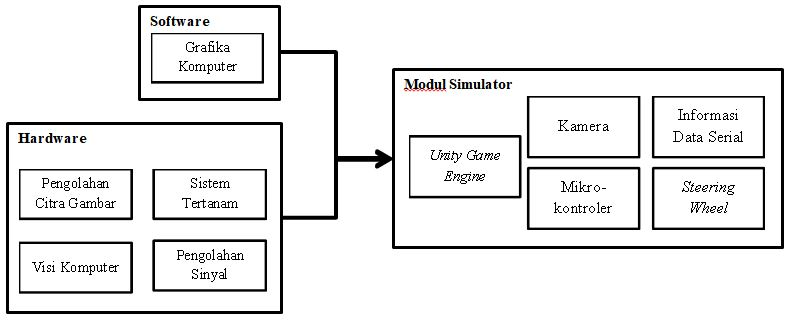
\includegraphics[scale=0.55]{img/cakupanTA.JPG}
	\caption{Blok Diagram Cakupan Disiplin Ilmu Tugas Akhir}
	\label{fig: 3_1}
\end{figure}
\vspace{1ex}
    \subsection{Cakupan \textit{Hardware}}
    Desain sistem secara umum pada gambar \ref{fig: 3_1}, yang mencakup disiplin ilmu perangkat keras atau \textit{hardware}, ialah pengolahan citra gambar, visi komputer, sistem tertanam, serta pengolahan sinyal. Disiplin pengolahan citra gambar didapatkan dari pengambilan citra pengemudi menggunakan kamera, visi komputer didapatkan dari proses \textit{recognition} wajah pengemudi, sistem tertanam atau \textit{embedded system} didapatkan dari komunikasi data - data serial menggunakan Arduino atau Mikroprosesor yang tersambung dengan simulator, kemudian yang terakhir Pengolahan sinyal didapatkan dari pengolahan data - data analog seperti data \textit{Electroencephalography (EEG)} / detak jantung pengemudi, atau data \textit{Electrooculography (EOG)} / data kedipan mata dari pengemudi.
    
    \subsection{Cakupan \textit{Software}}
   Cakupan Tugas Akhir ini pada bagian perangkat lunak atau \textit{software}, lebih ditekankan dalam upaya pembuatan \textit{Simulation Environment} atau Lingkungan Simulasi menggunakan \textit{Unity Game Engine}. \textit{Simulation Environment} dibuat dengan menggunakan disiplin ilmu grafika komputer 3d (3d \textit{Computer Graphics}), serta juga menggunakan proses - proses pengembangan dari \textit{game engine} dan \textit{physics engine} yang lain.
    
    \subsection{\textit{Output yang diharapkan}}
    \textit{Output} atau keluaran yang diharapkan dari tugas akhir ini ialah, dihasilkannya suatu modul simulasi yang terintegrasi lengkap dengan \textit{tools - tools} dan \textit{peripheral} yang yang dapat mensimulasikan suatu pengalaman mengemudi menggunakan suatu \textit{simulator}, serta dapat melakukan proses pengambilan data - data primer yang valid, sehingga dapat diolah untuk proses riset selanjutnya.


\section{Desain Sistem}
\vspace{1ex}
	Pada Tugas Akhir ini, dilakukan penggabungan perangkat lunak berupa \textit{game engine} untuk mensimulasikan proses berkendara, dengan perangkat keras berupa \textit{controller} dari \textit{simulator} dan \textit{Microcontroller} untuk proses pengambilan data. Proses kerja dari sistem ini akan dijelaskan melalui diagram alur pada gambar \ref{fig: 3_2}.
	Selain itu, simulator ini memiliki 2 jenis data yang dapat diukur. Berikut penjelasan 2 macam jenis data tersebut.
\begin{figure}  [!htb]
	\captionsetup{justification=centering}
	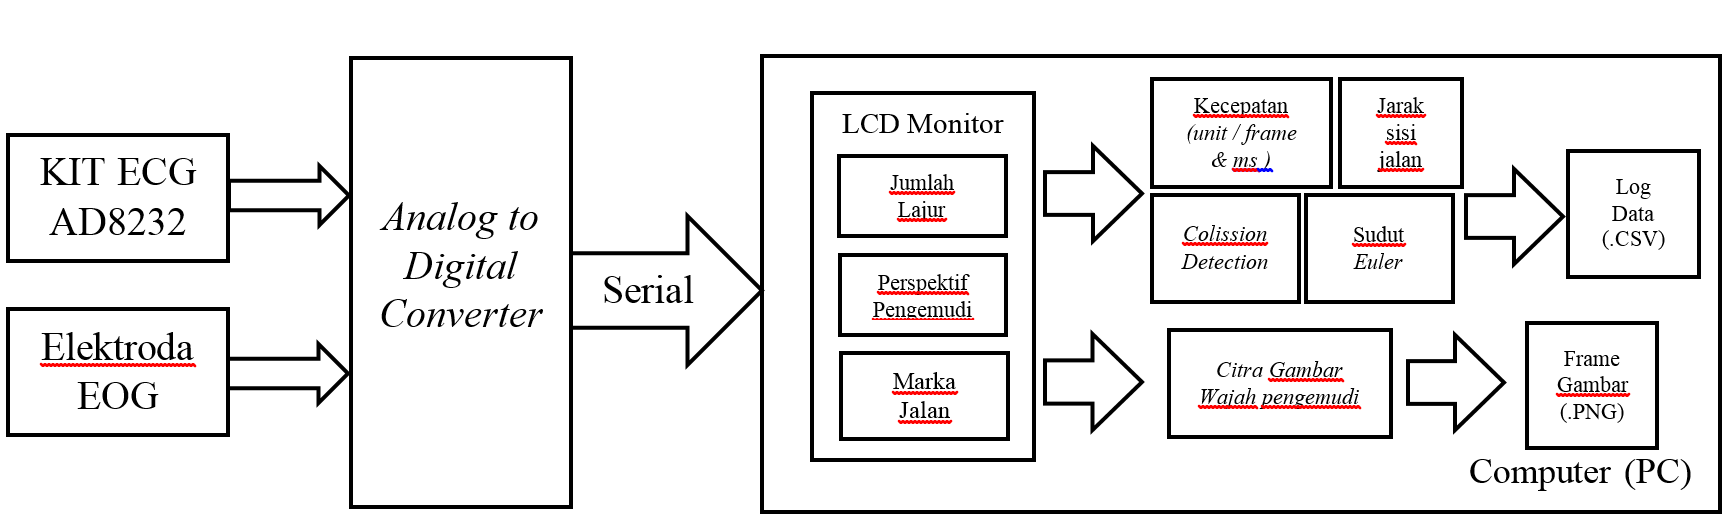
\includegraphics[scale=0.25]{img/desainsistem.PNG}
	%\caption{Diagram alur kerja}
	\caption{Desain umum modul Simulator}
	\label{fig: 3_2}
\end{figure}
\vspace{1ex}

    \subsection{Data - Data Internal Simulator}
    \vspace{1ex}
    Jenis data yang pertama adalah data yang berasal dari dalam modul simulator, yaitu data - data seperti kecepatan mobil, informasi spasial seperti, sudut \textit{euler} \textit{(pitch,yaw,roll)} dan jarak relatif terhadap pinggir jalan, informasi tabrakan / \textit{colission}, serta informasi waktu respon / \textit{response time}. Data - data ini, disebut sebagai data internal, dikarenakan data - data tersebut bisa di ekstraksi langsung dari \textit{game engine}.
    
        \subsubsection{Kecepatan Mobil / \textit{Velocity}}
        
        Pada unity game engine, menggunakan library Unity. Bisa didapatkan secara langsung variabel - variabel yang berhubungan dengan kecepatan. Pada tugas akhir ini, dibutuhkan data kecepatan mobil relatif terhadap dunia atau biasa disebut \textit{global velocity}. Namun selanjutnya, data kecepatan global pun bisa dibagi menjadi 4 macam, yaitu : \textit{velocity} atau kecepatan kearah sumbu \textit{x}, \textit{velocity} atau kecepatan kearah sumbu \textit{y}, serta \textit{velocity} atau kecepatan kearah sumbu \textit{z}, ketiga hal tersebut bisa juga disebut kecepatan vektor \textit{x,y,z}. Dan yang terakhir, adalah \textit{velocity magnitude}, atau tingkat kebesaran suatu kecepatan berupa skalar. Contoh data ini bisa dilihat pada tabel pengujian \ref{tb:4_2}
        
        \subsubsection{Informasi Spasial}
        
        \begin{figure}  [!htb]
	        \captionsetup{justification=centering}
	        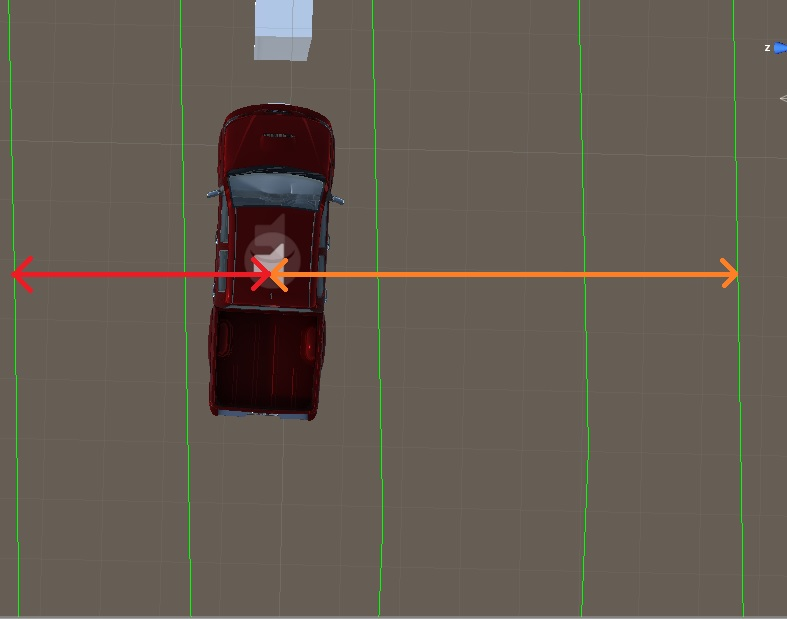
\includegraphics[scale=0.5]{img/relative-dist.jpg}
	        \caption{\textit{Relative Distance} \\ Oranye : Jarak dari \textit{Center of Mass} Mobil ke Batas Pinggir Kanan Jalan \\ Merah : Jarak dari \textit{Center of Mass} Mobil ke Batas Pinggir Kiri Jalan}
	        \label{fig: 3_19}
        \end{figure}
        
        Selain kecepatan, bisa didapatkan pula informasi spasial yang ada pada simulator. Pada tugas akhir ini, informasi spasial simulator adalah sudut euler yang merepresentasikan 6 derajat kebebasan atau biasa disebut \textit{6 Degree of Freedom (DoF))}, yaitu \textit{pitch, yaw,} dan \textit{roll} (gambar \ref{fig: 3_18}). Pada Tugas akhir ini, ketiga macam rotasi atau derajat kebebasan seluruhnya dimanfaatkan pada proses pembuatan desain jalan.
        
        \par Selanjutnya data spasial yang bisa didapatkan ialah posisi relatif kendaraan terhadap pinggir jalan (gambar \ref{fig: 3_19}). Dengan mengukur jarak terdekat dari titik pusat masa atau \textit{Center of Mass} mobil, ke batas pinggir kanan dan batas pinggir kiri jalan, dapat diketahui dimana posisi mobil di suatu lajur tersebut.
        
        \par Dengan menggabungkan dua macam jenis data tersebut, bisa didapatkan informasi yang sangat jelas tentang posisi dan orientasi dari kendaraan pengujian simulator ini. Yang nanti kedepannya sangat dibutuhkan untuk proses riset selanjutnya, yang akan memanfaatkan data - data tersebut.
        
        \subsubsection{Response Time}
        
        \begin{figure}  [!htb]
	        \captionsetup{justification=centering}
	        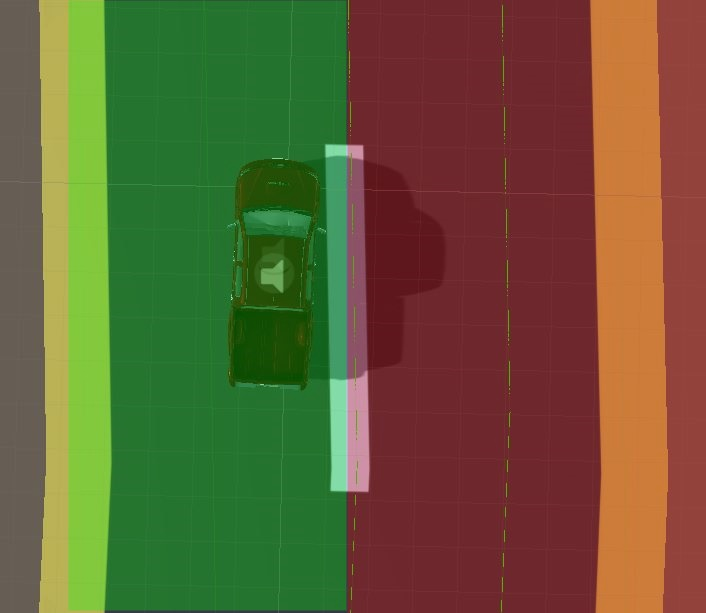
\includegraphics[scale=0.5]{img/jalur-tnp-mobil.JPG}
	        \caption{Response Time - IlustrasiJalur yang diharapkan - Kasus Tidak ada Mobil Lain}
	        \label{fig: 3_20}
        \end{figure}
        
        \begin{figure}  [!htb]
	        \captionsetup{justification=centering}
	        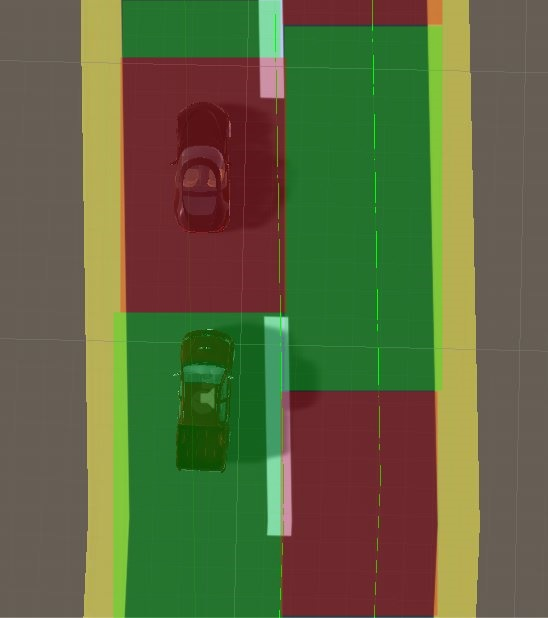
\includegraphics[scale=0.6]{img/jalur-dgn-mobil.JPG}
	        \caption{Response Time - Ilustrasi Jalur yang diharapkan - Kasus terdapat mobil lain}
	        \label{fig: 3_21}
        \end{figure}
        
        \textit{Response time} adalah metode pengukuran tingkat kewaspadaan pengemudi, dengan cara mendeteksi ketika pengemudi keluar dari lajur yang diharapkan. Lajur yang diharapkan disini, yang dimaksud ialah lajur sebelah kiri, dikarenakan desain simulator menggunakan model jalan yang ada di Indonesia. Berikut penjelasan tentang data \textit{Response time} pada gambar \ref{fig: 3_20} dan \ref{fig: 3_21}.
        
        Pada gambar \ref{fig: 3_20}, adalah gambar ilustrasi jalur yang diharapkan, pada kasus dimana tidak ada mobil lain didekat mobil pengujian. Warna hijau menandakan area yang di tandai oleh sistem simulator sebagai jalur yang diharapkan oleh sistem, artinya sistem mendeteksi bahwa mobil pada jalur yang telah sesuai serta pengemudi masih dalam keadaan waspada serta memiliki kontrol terhadap mobil. Apabila sistem mendeteksi mobil memasuki area yang berwarna merah, maka sistem akan melakukan pencatatan data yaitu kapan mobil mulai keluar dari jalur (tanggal dan waktu). Selanjutnya, sistem juga akan melacak mobil apabila mobil telah kembali ke area hijau, yang mana pada saat ini, sistem akan melakukan pencatatan data seberapa lama mobil telah keluar dari area hijau dengan \textit{unit} sekon, yang selanjutnya bisa didapatkan pula, seberapa lama mobil telah keluar dari area hijau dalam \textit{unit} hitungan \textit{frame}, dengan cara mengalikan waktu dalam sekon, dengan \textit{average framerate} dari simulator saat itu.
        
        \par Selanjutnya, pada gambar \ref{fig: 3_21}, adalah ilustrasi kasus dimana terdapat mobil didekat mobil uji, yang menyebabkan berubahnya jalur yang diharapkan. Apabila sistem mendeteksi terdapat mobil lain didekat mobil uji, sistem akan melakukan perubahan jalur yang diharapkan oleh sistem, metode penerapan pendeteksian seperti ini dapat diterapkan dengan banyak cara, salah satunya bisa dilakukan dengan membuat \textit{trigger box colission} disekitar mobil uji, yang mana ukurannya lebih besar dari \textit{bounding box} / ukuran mobil uji. Apabila terdapat suatu objek (seperti mobil lain), yang memasuki \textit{trigger box colission} dari mobil uji, maka bisa dilakukan perubahan pendeteksian jalur. Pada Tugas Akhir ini, digunakan metode ini untuk mendeteksi adanya mobil lain disekitar mobil uji, serta mendeteksi perlu terjadinya perubahan jalur yang diharapkan.
        
        \par Cara lain yang lebih mudah, namun tentunya dengan mengorbankan tingkat keakurasian pendeteksian yaitu adalah, dengan mengukur jarak mobil uji dengan mobil lain. Apabila jarak mobil uji dengan mobil lain ini dibawah nilai threshold, maka bisa dilakukan perubahan jalur yang diharapkan.
        
        \par Selanjutnya perlu digaris bawahi, bahwa sistem deteksi perubahan jalur ini juga sangat berkaitan dengan sistem deteksi terjadinya tabrakan. Sistem pendeteksian dan pencatatan data atau \textit{logging} dari \textit{colission event} ini akan dijelaskan pada subsubbab selanjutnya.
        
        \subsubsection{\textit{Colission Event}}
        
        \begin{figure}  [!htb]
	        \captionsetup{justification=centering}
	        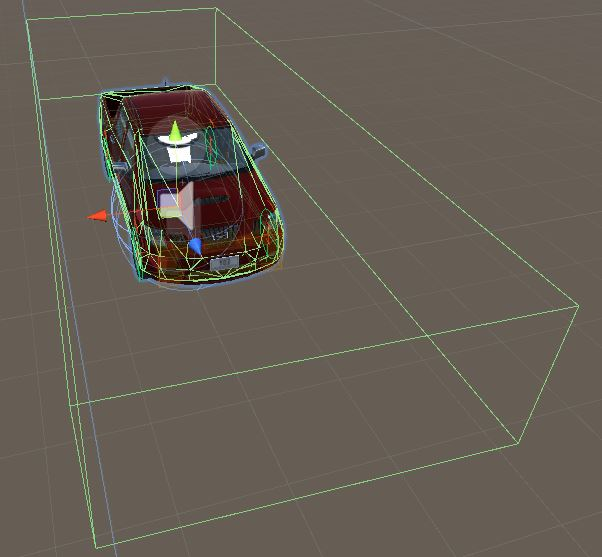
\includegraphics[scale=0.65]{img/colliders.JPG}
	        \caption{2 Macam \textit{Colliders} Mobil - \textit{Box Collider} dan \textit{Mesh Collider}}
	        \label{fig: 3_22}
        \end{figure}
        
        \begin{figure}  [!htb]
	        \captionsetup{justification=centering}
	        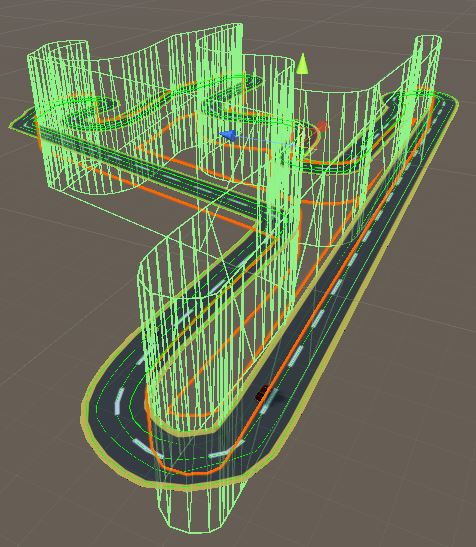
\includegraphics[scale=0.7]{img/boundary-inside.JPG}
	        \caption{\textit{Boundary} dalam sirkuit}
	        \label{fig: 3_23}
        \end{figure}
        
        \begin{figure}  [!htb]
	        \captionsetup{justification=centering}
	        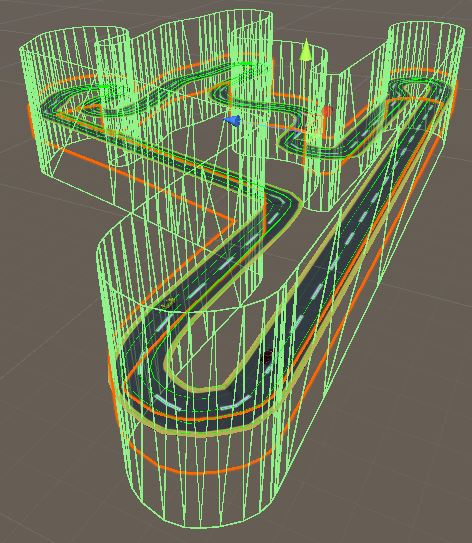
\includegraphics[scale=0.7]{img/boundary-outside.JPG}
	        \caption{\textit{Boundary} luar sirkuit}
	        \label{fig: 3_24}
        \end{figure}
        
         Pada subsubbab sebelumnya telah dijelaskan metode untuk mendeteksi keberadaan mobil lain di dekat mobil uji pada tugas akhir ini, yaitu dengan cara menggunakan \textit{trigger box event}. Pada subsubbab ini, \textit{colission event} yang dimaksud terdapat 2 macam. Yaitu yang pertama adalah, kejadian tabrakan dengan mobil lain, yang kedua kejadian tabrakan dengan pinggir jalan / \textit{boundary}. 
         
         \par Untuk proses pendeteksian tabrakan dengan mobil lain, dapat menggunakan \textit{mesh collider} yang sudah tersedia dengan mobil, untuk mempermudah proses deteksi, serta menyederhanakan \textit{physics interaction} antar mobil. Selain mobil uji, seluruh \textit{mesh collider} dari mobil lain ditentukan sebagai \textit{trigger}. Hal ini untuk menghindari terjadinya interaksi - interaksi yang tidak diinginkan ketika terjadi tabrakan antar mobil. 
         
         \par Dengan menggunakan fungsi \texttt{void onColissionEnter()} dan fungsi \texttt{void onTriggerEnter()} pada unity, dapat dilakukan pengecekan apabila terjadi overlap antar 2 \textit{GameObject} yang ada pada unity. Dengan menentukan \textit{GameObject} mana yang perlu dideteksi, sehingga langkah selanjutnya ialah mencatat data colission kedalam \textit{log file system}, 3 \textit{GameObject} yang perlu dideteksi adalah : \textit{Boundary} Luar / Batas Pinggir Kanan Jalan, \textit{Boundary} Dalam / Batas Pinggir Kiri Jalan, serta Mobil lain.
         
         \par Contoh data yang diambil pada \textit{colission event} bisa dilihat pada tabel \ref{tb:4_5}.
        
    
    \subsection{Data - Data Eksternal Simulator}
    \vspace{1ex}
    
     Selanjutnya Jenis data yang kedua adalah data yang berasal dari luar modul simulator, yaitu data - data seperti sinyal \textit{Electroencephalography (EEG)} / detak jantung pengemudi, dan atau data sinyal \textit{Electrooculography (EOG)} / data kedipan mata dari pengemudi, serta data citra wajah pengemudi menggunakan kamera. Data - data tersebut diatas, dikatakan sebagai data eksternal dikarenakan data - data tersebut didapatkan dari peralatan \textit{peripheral} yang dipasang pada modul simulator. Berhubung data EEG dan EOG merupakan data sinyal analog, maka diperlukannya suatu \textit{Analog to Digital Converter} atau ADC, supaya data bisa di rekam dalam \textit{log file}.
     Tentunya, perlu diperhatikan juga sampling rate dari ADC ini, sehingga bisa relevan dan dapat disesuaikan dengan data - data yang lain.
     
        \subsubsection{\textit{Serial Communication} Melalui \textit{port} COM}
        Pada tugas akhir ini, \textit{serial communication} melalui \textit{port} COM, dilakukan menggunakan \textit{Python}. Diagram \textit{flow chart} dari proses komunikasi data serial arduino ke PC, bisa di lihat pada gambar \ref{fig: 3_25}.
        \par Proses dari modul pembacaan data serial dimulai dengan pembuatan \textit{file} dengan nama tanggal dijalankannya modul tersebut. Hal ini dilakukan untuk mengetahui kapan waktu dan tanggal modul pembacaan dijalankan. Selain itu, hal ini memastikan bahwasanya file - file dapat dipisahkan atau disortir berdasarkan waktu dan tanggal, yang artinya data - data yang dicatat, tidak akan bercampur aduk dengan data - data percobaan yang sebelumnya.
        \par Dengan mengasumsikan bahwa arduino akan melakukan pengiriman data, \textit{python} akan terus membaca data dari arduino, dengan maksimum \textit{baudrate} yang telah ditentukan. Kemudian, setelah proses pembacaan dilakukan, akan dilakukan proses \textit{decode}. Proses \textit{Decode} ialah proses dimana \textit{python} akan melakukan konversi data biner, menjadi data - data diskrit \textit{integer} / bilangan bulat, yang kemudian hasil dari proses \textit{decode}, akan dilakukan proses append pada \textit{file} yang telah dibuat sebelumnya. 
        \par Informasi lebih jelas tentang proses \textit{append file} dan \textit{log file system} akan dijelaskan lebih lanjut pada sub-bab \ref{logfilesystem}
        
        \subsubsection{Citra Wajah Pengemudi / \textit{Webcam}}
        Pada \textit{Unity Game Engine}, sistem mensupport pembacaan informasi kamera webcam sebagai salah satu bagian dari \textit{library mobile camera information}, yang artinya adalah, apabila platform dari simulator menggunakan PC dengan OS \textit{Windows}, dan terdapat \textit{peripheral Webcam} yang terpasang, Unity dapat mendeteksi \textit{webcam} tersebut sebagai \textit{Imaging Device}.
        \par Sebagai \textit{Imaging Device}, data yang diperoleh unity dari \textit{webcam} ditangkap sebagai \textit{texture information}, atau informasi texture dari suatu \textit{GameObject}.
        
        \begin{figure}  [!htb]
	        \captionsetup{justification=centering}
	        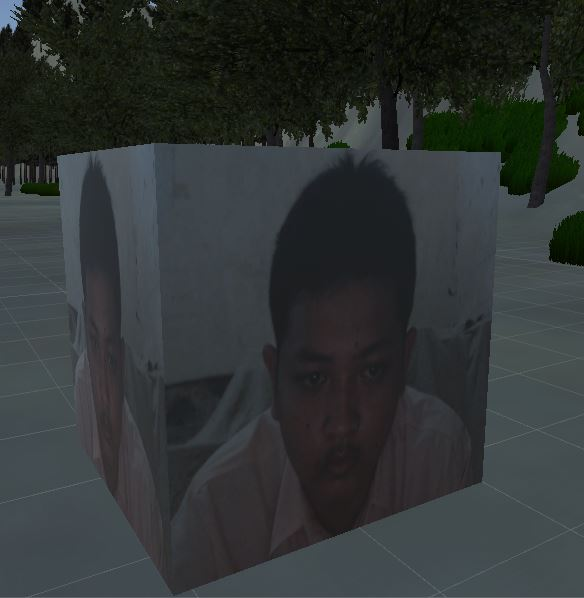
\includegraphics[scale=0.62]{img/webcam-texture.JPG}
	        \caption{Kubus yang memiliki \textit{texture information} dari \textit{Webcam / Imaging Device}}
	        \label{fig: 3_26}
        \end{figure}
        
       Dikarenakan informasi yang ditangkap oleh unity merupakan suatu \textit{texture}, maka \textit{texture} tersebut bisa di pasangkan ke suatu \textit{GameObject}, agar memiliki tampilan dari \textit{webcam}.  Bisa dilihat, pada gambar \ref{fig: 3_26}, ketika informasi webcam di pasangkan dengan kubus.
       \par Namun pada tugas akhir ini, yang dibutuhkan bukanlah informasi \textit{texture} yang bisa digunakan oleh game ini. Yang dibutuhkan adalah \textit{frame - frame} / gambar wajah dengan \textit{timestamp} yang sesuai. Maka langkah selanjutnya adalah mengekstrak informasi \textit{texture} tersebut keluar dari unity. Hal ini mudah dilakukan dengan melakukan fungsi \textit{encoding} ke tipe \textit{file} yang berekstensi \textit{PNG}. Setelah encoding dilakukan, \textit{file stream} akan menuliskan data hasil \textit{encoding} menjadi suatu gambar lengkap dengan \textit{timestamp} nya.
       \par Hasil pengujian pengambilan data citra wajah pengemudi menjadi frame - frame yang telah di \textit{encode} menjadi PNG bisa di lihat pada gambar \ref{fig:4.2}
    
\section{Desain Lajur Simulator}
\vspace{1ex}

    \par Pada tugas akhir ini, terdapat 4 macam lajur yang dapat dipilih oleh pengemudi. 4 Macam lajur tersebut berfungsi sebagai basis riset untuk mengeliminasi terjadinya bias atau pengaruh yang dihasilkan oleh perbedaan jumlah lajur yang digunakan.
    
\begin{figure}  [!htb]
	\captionsetup{justification=centering}
	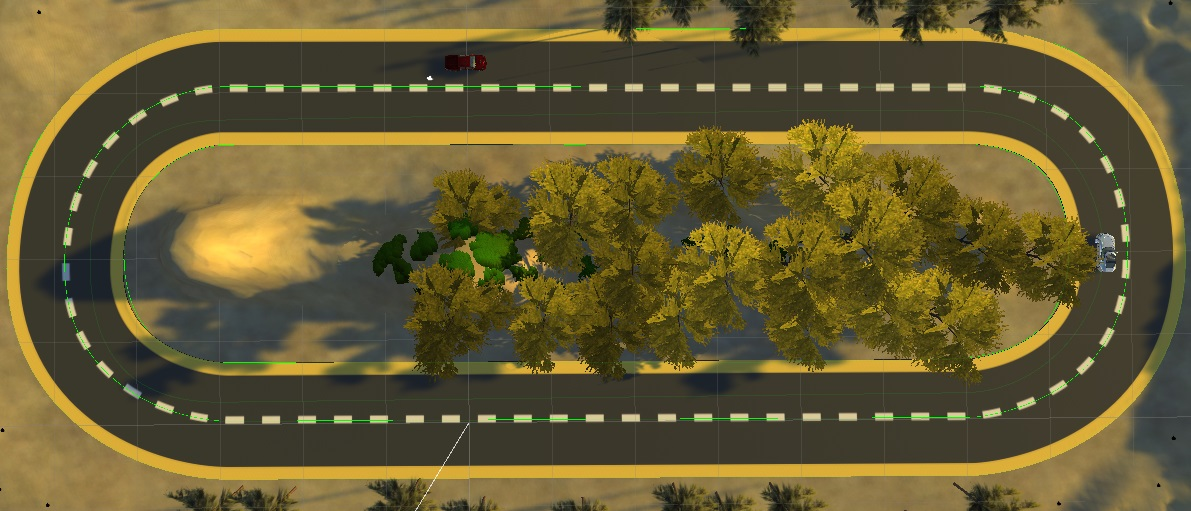
\includegraphics[scale=0.31]{img/2lj_short_oh.jpg}
	\caption{Desain sirkuit 2 lajur dengan jarak yang pendek dan kompleksitas yang rendah}
	\label{fig: 3_3}
\end{figure}
\vspace{1ex}

\begin{figure}  [!htb]
	\captionsetup{justification=centering}
	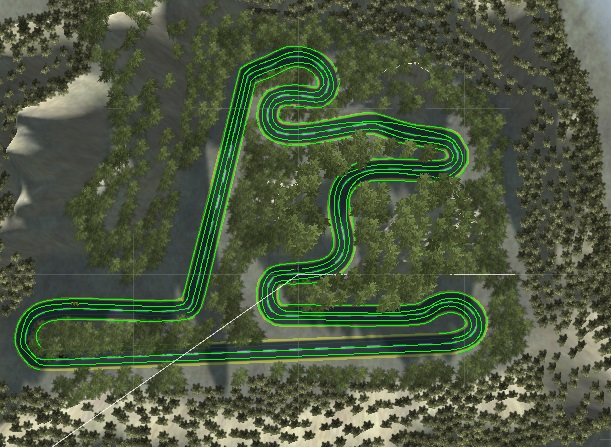
\includegraphics[scale=0.53]{img/2lj_long_oh.jpg}
	\caption{Desain sirkuit 2 lajur dengan jarak yang panjang dan kompleksitas yang tinggi}
	\label{fig: 3_4}
\end{figure}
\vspace{1ex}

\begin{figure}  [!htb]
	\captionsetup{justification=centering}
	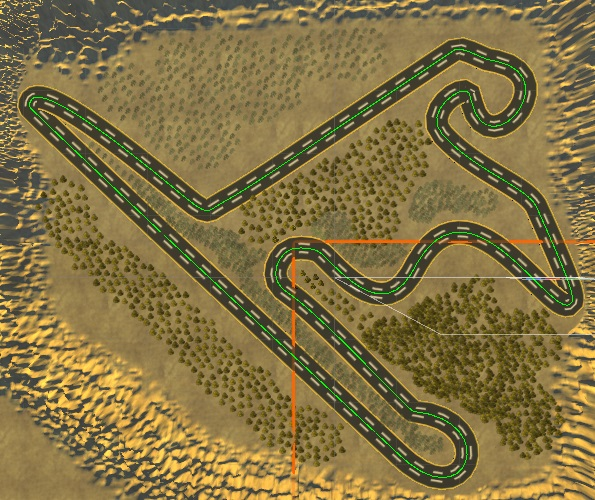
\includegraphics[scale=0.53]{img/3lj_oh.jpg}
	\caption{Desain sirkuit 3 lajur}
	\label{fig: 3_5}
\end{figure}
\vspace{1ex}

\begin{figure}  [!htb]
	\captionsetup{justification=centering}
	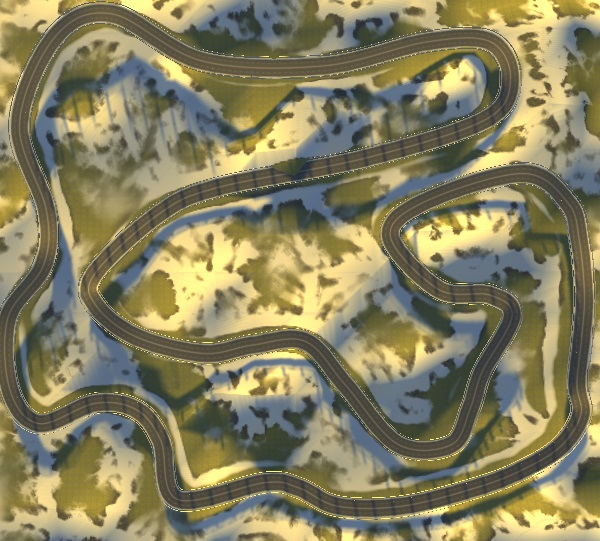
\includegraphics[scale=0.53]{img/4lj_oh.jpg}
	\caption{Desain sirkuit 4 lajur}
	\label{fig: 3_6}
\end{figure}
\vspace{1ex}

    \par Berikut pada Gambar \ref{fig: 3_3}, \ref{fig: 3_4}, \ref{fig: 3_5}, dan \ref{fig: 3_6}, adalah tampak atas dari desain - desain lajur yang digunakan pada simulator ini, seluruh lajur didesain dengan bentuk \textit{closed-loop circuit}. Hal ini bertujuan agar mengurangi ukuran aset jalan yang akan digunakan. Selain itu desain seperti ini dapat berdampak pada durasi pengambilan data, desain sirkuit yang \textit{closed-loop} memungkinkan kegiatan proses pengambilan data supaya tidak bergantung pada panjang jalan yang digunakan.
    \par Tabel \ref{tb:3_1} adalah detil informasi dari desain jalan / sirkuit yang dibuat pada simulator ini. 
    
\begin{table}[]
\caption{Tabel Informasi Sirkuit Jalan}
\label{tb:3_1}
\begin{tabular}{|c|c|c|c|c|c|}
\hline
\multirow{2}{*}{No.} & \multirow{2}{*}{\begin{tabular}[c]{@{}c@{}}Jumlah Lajur\\ (Unit)\end{tabular}} & \multirow{2}{*}{\begin{tabular}[c]{@{}c@{}}Jarak\\ (Unit)\end{tabular}} & \multirow{2}{*}{\begin{tabular}[c]{@{}c@{}}Lebar\\ (Unit)\end{tabular}} & \multicolumn{2}{c|}{\begin{tabular}[c]{@{}c@{}}Kompleksitas\\ (Tampak Atas)\end{tabular}} \\ \cline{5-6} 
                     &                                                                                &                                                                         &                                                                               & \textit{CW Curve}                           & \textit{CCW Curve}                          \\ \hline
1                    & 2                                                                              & 43,145                                                                  & 12                                                                            & 4                                           & 0                                           \\ \hline
2                    & 2                                                                              & 260.226                                                                 & 12                                                                            & 6                                           & 10                                          \\ \hline
3                    & 3                                                                              & \multicolumn{1}{l|}{260.226}                                            & 16                                                                            & 6                                           & 10                                          \\ \hline
4                    & 4                                                                              & 411.346                                                                 & 20                                                                            & 11                                          & 12                                          \\ \hline
\end{tabular}
\end{table}
    
\section{Desain \textit{Behaviour} dari Kendaraan Lain}
\vspace{1ex}

    \par Pada Tugas akhir ini, Desain dari \textit{AI Behavior} kendaraan lain cukup mengikuti lajur sirkuit sesuai dengan jalur yang telah didefinisikan oleh \textit{Bézier curve}, kemudian pada script \textit{follower} yang ada di unity, dikarenakan desain lajur yang \textit{closed-loop}, perlu di definisikan arah dari kendaraan tersebut, dilihat dari tampak atas, apakah kendaraan memiliki \textit{clockwise path} atau \textit{counter-clockwise path}.
    \par Selain arah dari kendaraan, diperlukannya pendefinisian kecepatan kendaraan tersebut, pada Tugas Akhir ini kecepatan kendaraan ditentukan dengan randomisasi dalam suatu rentang tiap kali simulator dijalankan.
    \par Informasi detil dari desain AI kendaraan lain di \textit{unity}, dapat dilihat pada tabel \ref{tb:3_2}

\begin{table}[]
\caption{Tabel Informasi AI Tiap - Tiap Tipe Lajur}
\label{tb:3_2}
\begin{tabular}{|c|c|c|c|c|c|c|}
\hline
\multirow{2}{*}{No.} & \multirow{2}{*}{Lajur} & \multirow{2}{*}{\begin{tabular}[c]{@{}c@{}}Jumlah\\ Mobil\end{tabular}} & \multicolumn{2}{c|}{\textit{AI Rotation}}             & \multicolumn{2}{c|}{\textit{\begin{tabular}[c]{@{}c@{}}Velocity\\ (Unit/Frame)\end{tabular}}} \\ \cline{4-7} 
                     &                        &                                                                         & \textit{CW}               & \textit{CCW}              & \textit{Min}                                  & \textit{Max}                                  \\ \hline
1                    & \textit{2 (Short)}     & 1                                                                       & \xmark     & \checkmark & 5.0f                                          & 15.0f                                         \\ \hline
2                    & \textit{2 (Long)}      & 2                                                                       & \checkmark & \checkmark & 0.1f                                          & 0.9f                                          \\ \hline
3                    & 3                      & 3                                                                       & \checkmark & \checkmark & 0.1f                                          & 0.9f                                          \\ \hline
4                    & 4                      & 4                                                                       & \checkmark & \checkmark & 0.01f                                         & 0.1f                                          \\ \hline
\end{tabular}
\end{table}

\section{Alur Kerja}
\vspace{1ex}

Pembuatan tugas akhir ini dibagi menjadi beberapa tahapan, yaitu:
    \begin{enumerate}[nolistsep]
	
	\item \nohyphens{Pembuatan Simulasi Menggunakan \textit{Unity Game Engine}}
	\item Pengaturan dan Konfigurasi \textit{Steering Wheel Controller} 
	\item Pembuatan Modul Pengambilan Data dengan \textit{Microcontroller}
	\item Penggabungan Seluruh Sistem Menjadi Satu Modul
	
	\end{enumerate}

\section{Pembuatan Simulasi Menggunakan \textit{Unity Game Engine}}
\vspace{1ex}
   Pada Tugas Akhir ini, proses pembuatan simulasi menggunakan \textit{Unity Game Engine}. Namun tidak hanya menggunakan \textit{Unity Game Engine} saja, tentunya selain memanfaatkan \textit{unity editor}, juga diperlukan \textit{source code editor}, pada tugas akhir ini menggunakan \textit{Visual Studio 2017}. Selain itu terdapat \textit{tools - tools} lain di luar \textit{unity} yang dapat mempermudah proses pembuatan Simulator ini.
	
	\subsection{Pembuatan Sirkuit Jalan}
	\vspace{1ex}
	
	\begin{figure} [!htb]
	    \captionsetup{justification=centering}
	    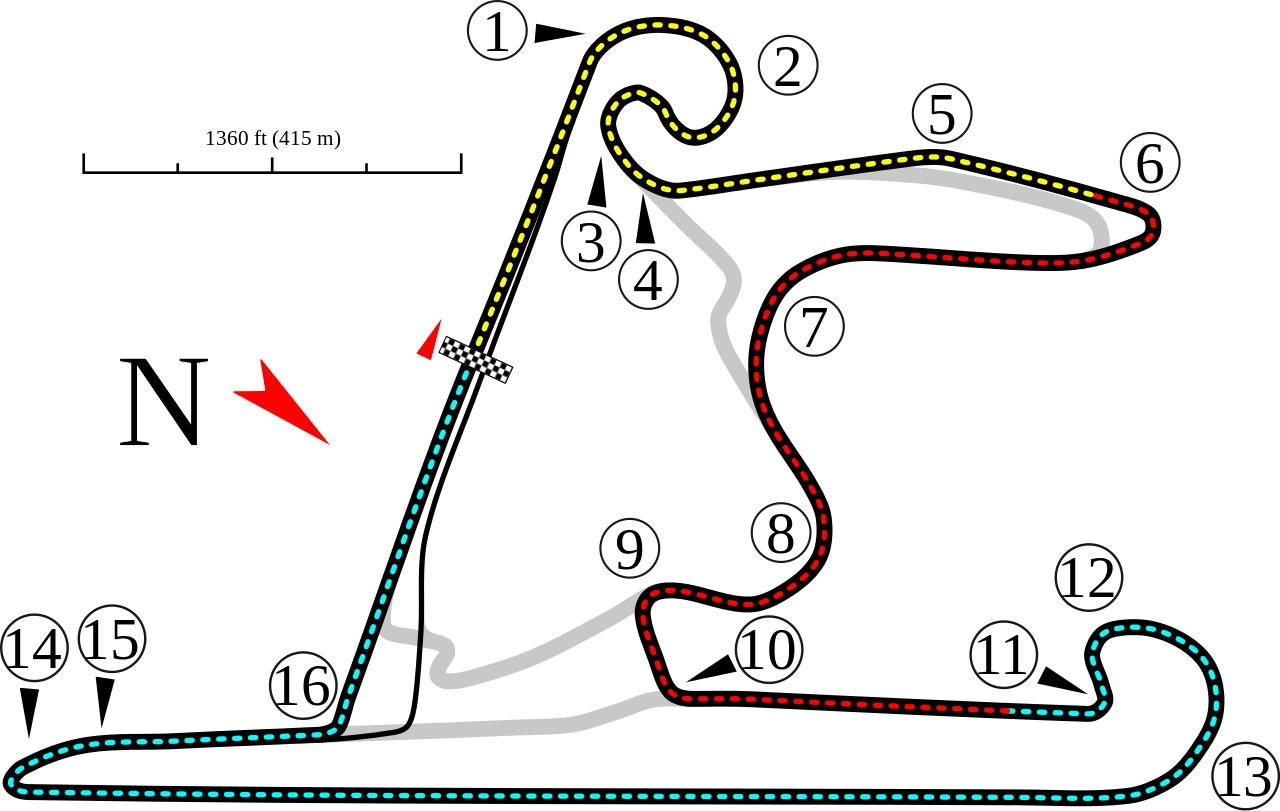
\includegraphics[scale=0.25]{img/shanghai-ic.png}
	    \caption{\textit{Shanghai International Circuit\cite{cit:14}}}
	    \label{fig: 3_10}
    \end{figure}
	
	\begin{figure} [!htb]
	    \captionsetup{justification=centering}
	    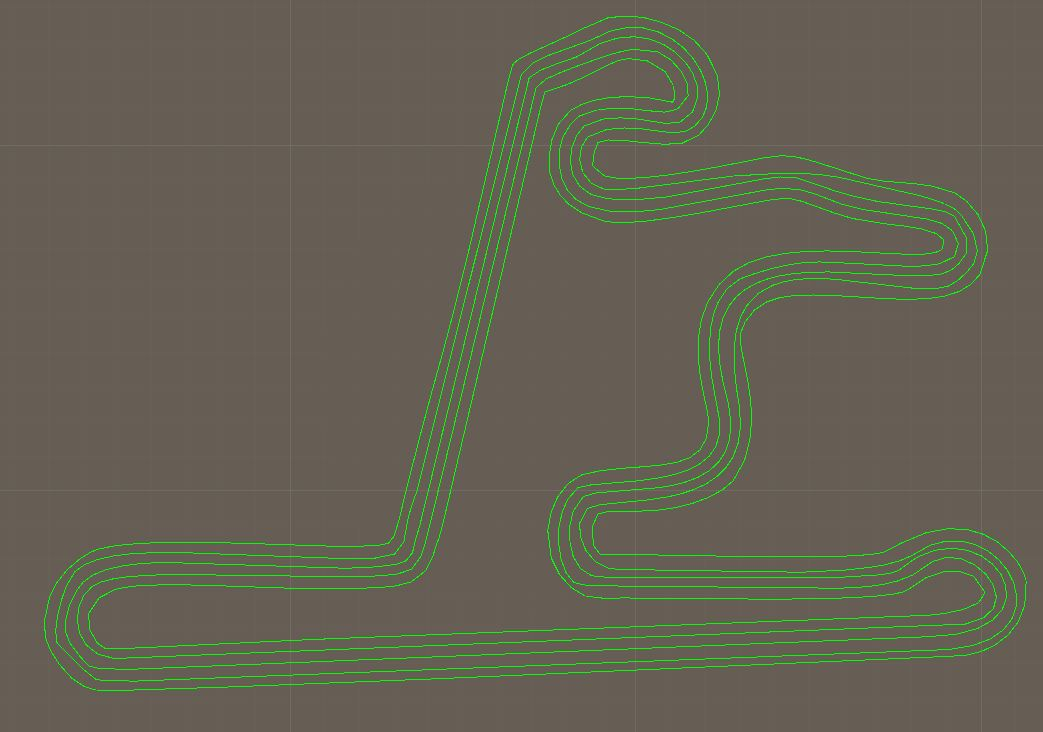
\includegraphics[scale=0.36]{img/bezier-curve-jalan.JPG}
	    \caption{5 Macam \textit{Bézier curve} sirkuit (dari kiri ke kanan) : batas kiri jalan, \textit{Vehicle AI Path - Counterclock Wise}, tengah lajur / marka jalan, \textit{Vehicle AI Path - Clock Wise}, serta batas kanan jalan }
	    \label{fig: 3_9}
    \end{figure}
	
	Proses pembuatan sirkuit jalan adalah proses yang paling memakan waktu pada tugas akhir ini. Yang pertama perlu dilakukan adalah mendefinisikan \textit{path} jalan menggunakan \textit{Bézier curve}, atau jalur yang akan digunakan sebagai \textit{base} dari \textit{3d mesh} jalan atau lajur itu sendiri, salah satu contohnya adalah pada gambar \ref{fig: 3_9}, bisa dilihat terdapat 5 macam kurva bezier yang dapat ditemukan. Semua 5 kurva tersebut dibutuhkan untuk proses kalkulasi informasi jarak serta informasi \textit{colission} yang nantinya akan disimpan kedalam \textit{log file}.
	\par Menggunakan \textit{Shanghai International Circuit} dari \textit{Formula 1}, sebagai referensi bentuk dari sirkuit, diperlukannya penyesuaian tingkat kelengkungan dari belokan yang ada pada sirkuit referensi. Untuk menghindari \textit{mesh overlap}, maka tiap - tiap tikungan yang tajam, perlu diperhalus sedemikian hingga \textit{mesh overlap} agar tidak terjadi. Namun tidak terlalu dikurangi sehingga pengemudi tetap waspada terhadap tikungan tersebut, serta supaya pengemudi mengurangi kecepatan sebelum melakukan belokan tersebut.
	\par Hal ini penting, dikarenakan pada saat proses pengujian berjalan, mobil tidak diharapkan untuk keluar dari lajur pengujian.
	    
	    \subsubsection{\textit{Editing Tools : Path Creator}}
	    \vspace{1ex}
	    
	    \begin{figure} [!htb]
	        \captionsetup{justification=centering}
	        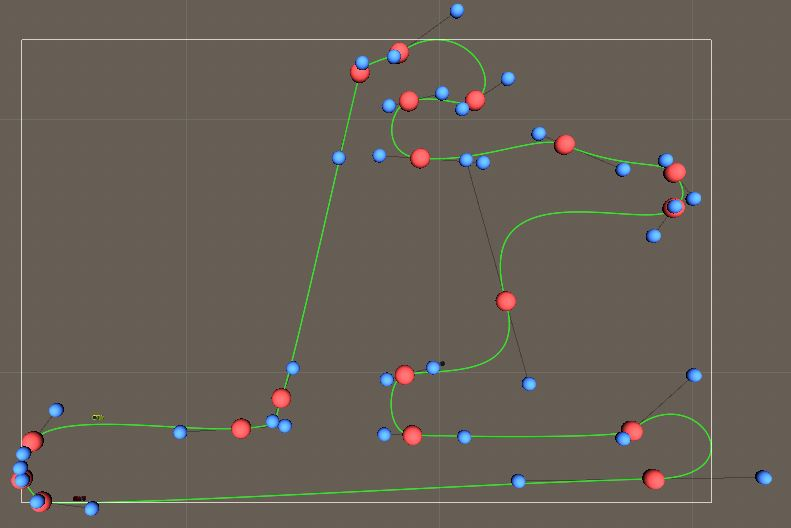
\includegraphics[scale=0.47]{img/bezier-curve-cp.JPG}
	        \caption{\textit{Bézier curve} tampak atas, merah : \textit{anchor points}, biru : \textit{control points}}
	        \label{fig: 3_11}
        \end{figure}
        
        \begin{figure} [!htb]
	        \captionsetup{justification=centering}
	        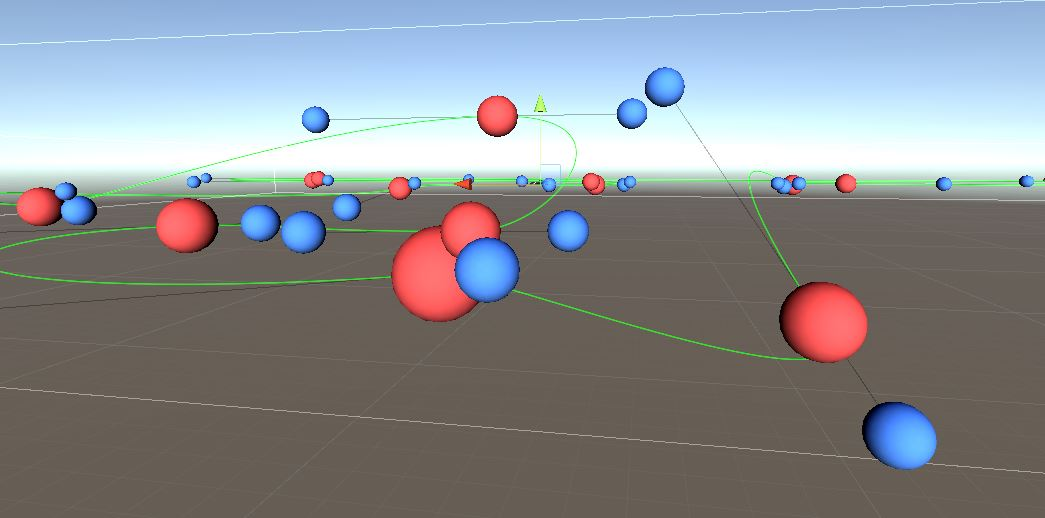
\includegraphics[scale=0.35]{img/bezier-curve-cp2.JPG}
	        \caption{\textit{Bézier curve} pada \textit{3d plane}}
	        \label{fig: 3_12}
        \end{figure}
	    
	    Untuk memudahkan proses pembuatan \textit{Bézier curve}, pada unity. Penulis menggunakan \textit{tools} yang tersedia di unity yang berfungsi untuk mempermudah kalkulasi matematis serta proses \textit{scripting} yang ada pada unity untuk menghasilkan kurva tersebut. Tools tersebut ialah \textit{Path Creator} oleh Sebastian Lague, Path Creator ini dipilih dikarenakan, memudahkan dalam proses manipulasi kurva \textit{Bézier}. Dikarenakan pada \textit{unity} tidak mensupport kurva \textit{Bézier} secara natif, maka biasanya para \textit{game developer}, membuat \textit{script} mereka masing - masing untuk membuat kurva \textit{Bézier}, dengan melakukan kalkulasi persamaan matematis pada script mereka tersebut, kemudian diperlukannya manipulasi titik - titik kontrol sesuai dengan \textit{script} tersebut.
	    \par Namun \textit{Path Creator} memungkinkan penulis untuk melewati proses kalkulasi matematis serta pendefinisian titik - titik kontrol, langsung ke proses manipulasi \textit{drag and drop} titik - titik kontrol, pada \textit{Unity Editor}.
	    \par Pada gambar \ref{fig: 3_11} dan \ref{fig: 3_12}, bisa dilihat titik - titik yang dapat dimanipulasi menggunakan \textit{Path Creator}. Warna merah menunjukkan \textit{anchor points}, yang artinya titik tersebut merupakan titik - titik statis pada suatu persamaan kurva, dengan memanipulasi lokasi dari \textit{anchor points} pada 3 dimensi, dapat didapatkan bentuk \textit{approximation} dari target sirkuit diinginkan. Tentunya, semakin banyak \textit{anchor points} yang digunakan, semakin akurat pula \textit{approximation} jalan yang dibuat. Namun tentunya, kurva jalan menjadi lebih kompleks serta lebih sulit untuk dimanipulasi.
	    \par Kemudian, warna biru menunjukkan \textit{control points}, \textit{control points} ini menentukan lengkungan yang diharapkan diantara tiap - tiap \textit{anchor points}, tentunya agar didapatkankannya lengkungan yang sesuai dengan belokan yang ada pada sirkuit referensi, titik - titik inilah yang akan dapat dimanipulasi.
	    
	    \subsubsection{\textit{Plane Projection} serta \textit{Normal Vector}}
        
        Pada Tugas Akhir ini, informasi tentang \textit{plane projection} yang ada pada kurva \textit{Bézier} sangat penting. Hal ini dapat menunjukkan informasi tentang kekasaran medan atau \textit{level} ketinggian dari suatu daerah pada \textit{terrain} yang ada pada jalan.
        
        \par Pada Tugas akhir ini, jalan yang memiliki 2 dan 3 lajur, memiliki \textit{plane projection} terhadap \textit{XZ Plane}, artinya medan yang ada pada kedua macam jumlah lajur tersebut memiliki kedataran yang seragam, tidak memiliki tanjakan ataupun turunan. 
        
        \par Sedangkan, pada jalan yang memiliki 4 lajur, dengan memanfaatkan semua sumbu \textit{XYZ} maka dapat dihasilkan jalur yang memiliki tanjakan dan turunan.
        
        \begin{figure} [!htb]
	        \captionsetup{justification=centering}
	        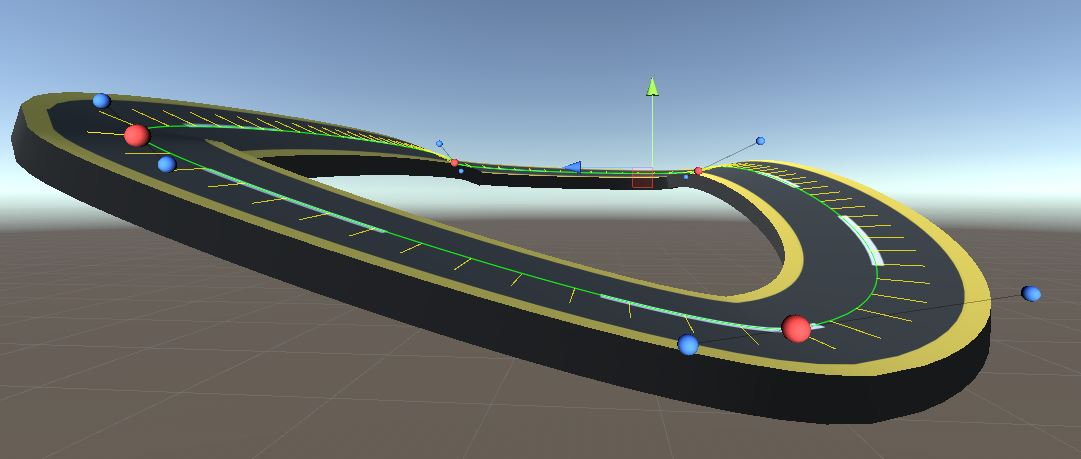
\includegraphics[scale=0.35]{img/pp1.JPG}
	        \caption{\textit{Normal Force} Jalan (\textit{Yaw} 0 Derajat)}
	        \label{fig: 3_13}
        \end{figure}
        
        \begin{figure} [!htb]
	        \captionsetup{justification=centering}
	        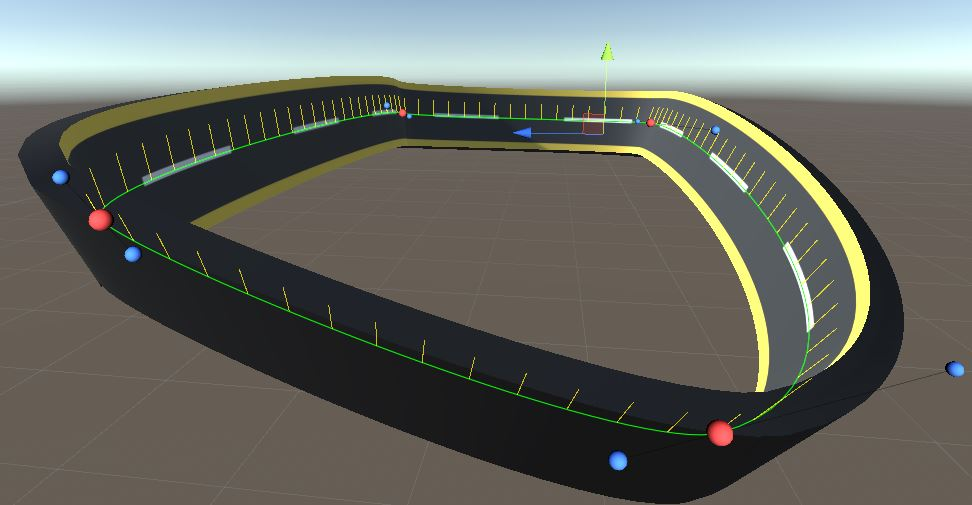
\includegraphics[scale=0.35]{img/pp2.JPG}
	        \caption{\textit{Normal Force} Jalan (\textit{Yaw} 60 Derajat)}
	        \label{fig: 3_14}
        \end{figure}
        
        Kemudian selanjutnya adalah, penentuan \textit{normal force}. Pada \textit{path creator}, parameter yang dapat dikontrol adalah \textit{global angle}, dari normal force tersebut. Hal ini menentukan sudut rotasi / \textit{yaw}, dari jalan yang dibuat pada path yang ditentukan.
        \par Berikut pada gambar \ref{fig: 3_13} dan gambar \ref{fig: 3_14}, perbandingan efek dari \textit{normal force} yang ada di jalan. Hal ini penting diperhatikan untuk proses desain serta pembuatan jalan, yang memanfaatkan seluruh 6 derajat kebebasan \textit{(Degree of Freedom)}, \textit{pitch, yaw,} dan \textit{roll}
	
	\subsection{Pembuatan \textit{Terrain}}
	\vspace{1ex}
	
	Medan atau \textit{terrain}, merupakan kanvas kosong dari sebuah \textit{scene}, yang dapat diisi dengan berbagai macam objek - objek estetis untuk meningkatkan realisme dan imersivitas pada proses simulasi. Pada tugas akhir ini medan yang dibuat pada tiap lajur tidak terlalu berpengaruh terhadap proses pengambilan data itu tersendiri, namun merupakan salah satu \textit{design choice} atau proses pemilihan desain agar meningkatkan kualitas dari \textit{user experience}.
	
	\par Setelah proses pembuatan jalan selesai, untuk meningkatkan estetika, diperlukannya \textit{terrain} yang mengelilingi jalan. Pada \textit{Unity,} objek - objek \textit{non-colission} dapat ditaruh untuk meningkatkan estetika tersebut. Seperti contohnya, pohon - pohon dan semak - semak atau rerumputan. Selain itu, dapat diterapkan perubahan kontur dari \textit{terrain}. Seperti contohnya dapat diterapkan proses peninggian sebagian dari \textit{terrain} untuk menghasilkan bukit, atau bahkan sebaliknya, proses penurunan dari sebagian \textit{terrain} dapat menghasilkan lembah.
	
    Selain itu, pada \textit{unity} dapat ditambahkannya tekstur pada \textit{terrain}. Tekstur disini yang dimaksud ialah, warna atau gambar yang dapat diterapkan pada \textit{terrain} agar menghasilkan corak pada \textit{terrain}. Seperti contohnya tekstur dari tanah coklat, atau tekstur warna pasir kuning, dan sebagainya.
    
    \begin{figure} [!htb]
	    \captionsetup{justification=centering}
	    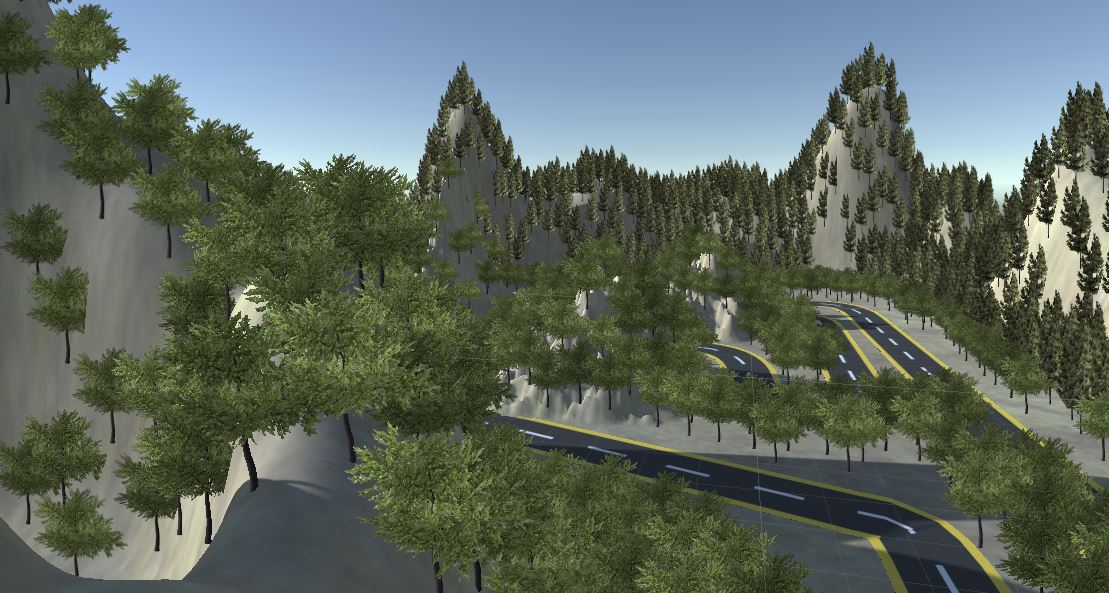
\includegraphics[scale=0.35]{img/terrain.JPG}
	    \caption{\textit{Terrain} setelah ditambahkan bukit, dan pepohonan}
	    \label{fig: 3_17}
    \end{figure}
    
    Selanjutnya, perlu di garis bawahi juga, pada Tugas Akhir ini, salah satu \textit{design choice} merupakan jalan berbentuk sirkuit, maka dari itu terrain, untuk mengakomodasi hal tersebut di terapkan bukit yang mengelilingi sirkuit jalan, untuk memberikan kesan bahwasanya mobil tidak dapat keluar dari lajur.
    
    \subsection{\textit{Menu} dan \textit{User Interface}}
    
    Proses pembuatan Menu dibutuhkan untuk memudahkan pemilihan jumlah lajur nanti setelah simulator menjalani proses \textit{build}. Menu disini dibutuhkan agar tidak terlalu kompleks, namun cukup agar menu dapat menjelaskan serta merepresentasikan tampilan atau tombol yang ditekan. Pemilihan yang intuitif serta fungsionalitas yang berjalan sudah cukup untuk proses ketika di menu.
    \par Perlu diperhatikan juga, dapat diterapkan pula \textit{asynchronous loading}, pada menu ini. Artinya, \textit{scene} atau jenis lajur yang dipilih, akan di muat sebelum tombol ditekan. Supaya proses \textit{loading} akan menjadi lebih cepat.
    
    \begin{figure} [!htb]
	    \captionsetup{justification=centering}
	    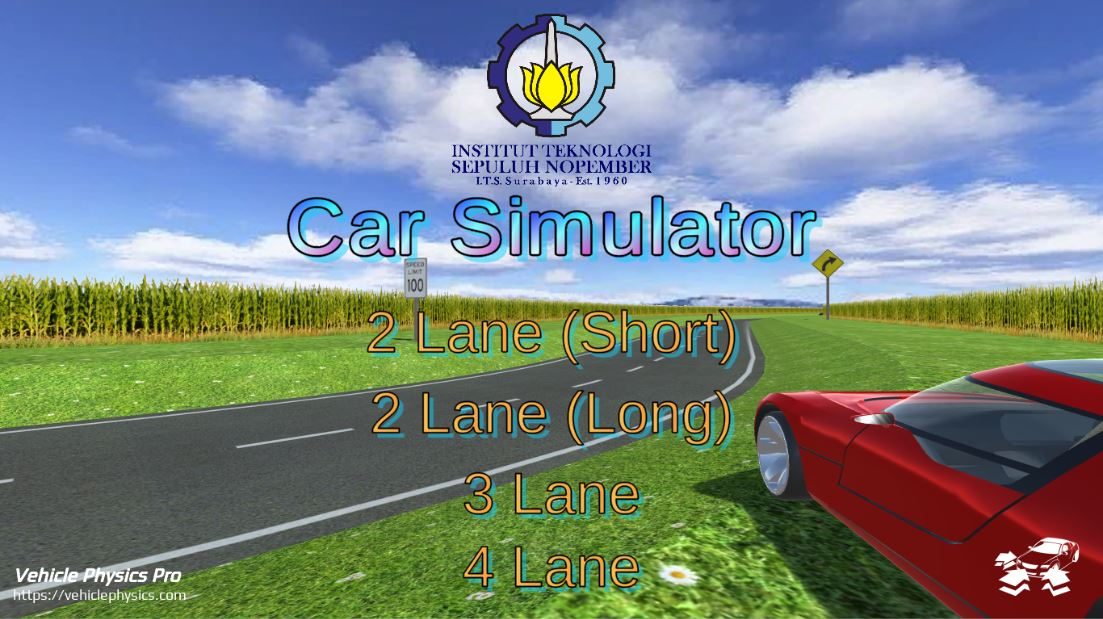
\includegraphics[scale=0.35]{img/menuUI.JPG}
	    \caption{\textit{User Interface} dari Menu}
	    \label{fig: 3_15}
    \end{figure}
    
    Gambar \ref{fig: 3_16} adalah, gambar yang menunjukkan hasil menu yang dibuat. Terdapat 4 tombol yang bisa ditekan, tiap - tiap tombol memiliki penjelasan \textit{text} yang jelas, yaitu merepresentasikan tombol yang akan membawa \textit{user} menuju \textit{scene} atau lajur yang sesuai dengan text tersebut, seperti 2 lajur pendek, 2 lajur panjang, 3 lajur, serta 4 lajur. Selain itu, dipasang pula \textit{background canvas} serta logo ITS pada \textit{User Interface} Menu.
    
    \subsection{\textit{Log File System} dan \textit{Kalkulasi Data}} 
    \label{logfilesystem}
    
    \textit{Log File System} adalah salah satu komponen penting dari Tugas Akhir ini, agar didapatkan suatu \textit{Log File System}, beberapa macam komponen dibutuhkan dari sistem ini (gambar \ref{fig: 3_15}).
    
    \begin{figure} [!htb]
	    \captionsetup{justification=centering}
	    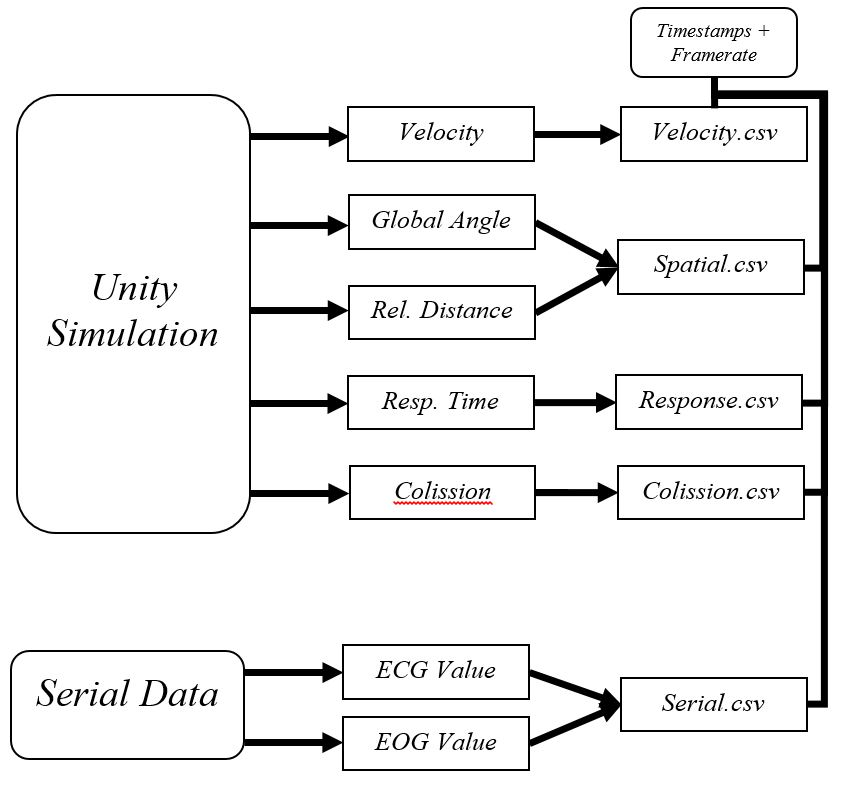
\includegraphics[scale=0.5]{img/logfile.JPG}
	    \caption{Diagram \textit{Log File System}, proses ekstraksi data, dan proses \textit{append data}}
	    \label{fig: 3_31}
    \end{figure}
    
    Yang pertama adalah, proses ekstraksi data. Proses ini sangat mudah dikarenakan informasi - informasi yang dibutuhkan sudah tersedia dan tertulis pada variabel - variabel yang dipakai pada simulasi serta komunikasi \textit{serial data}. 
    \par Setelah proses ekstraksi data yang dibutuhkan, selanjutnya dibuatlah komunikasi \textit{file stream} dari \textit{unity} ke \textit{OS file system}, pada Tugas Akhir ini, OS yang digunakan adalah Windows 8.1. Komunikasi file stream yang dibuat bertugas untuk mengecek apakah \textit{path} dari direktori yang dituju sudah ada, apabila belum tersedia folder yang diharapkan, maka \textit{file stream}, akan membuat folder pada direktori yang diinginkan dan membuat \textit{file - file} sesuai dengan \textit{output data} yang ada.
    \par Langkah selanjutnya adalah \textit{file stream} akan membuka \textit{file} yang telah dibuat tersebut, kemudian melakukan \textit{append}, atau penambahan data kedalam \textit{file} tersebut. Jenis \textit{Append} yang pertama kali dilakukan adalah melakukan \textit{append header}, atau informasi - informasi pada ujung tabel (label), serta informasi \textit{separator} dari kolom. Pada Tugas Akhir ini, seluruh \textit{output file}, menggunakan \textit{separator} kolom berupa \textit{tab} atau simbol \textit{\textbackslash t} sedangkan separator baris berupa \textit{line break} atau simbol \textit{\textbackslash n}
    

\section{Pengaturan dan Konfigurasi \textit{Steering Wheel Controller}}
\label{steeringwheelconf}
\vspace{1ex}
    \begin{figure}  [!htb]
	    \captionsetup{justification=centering}
	    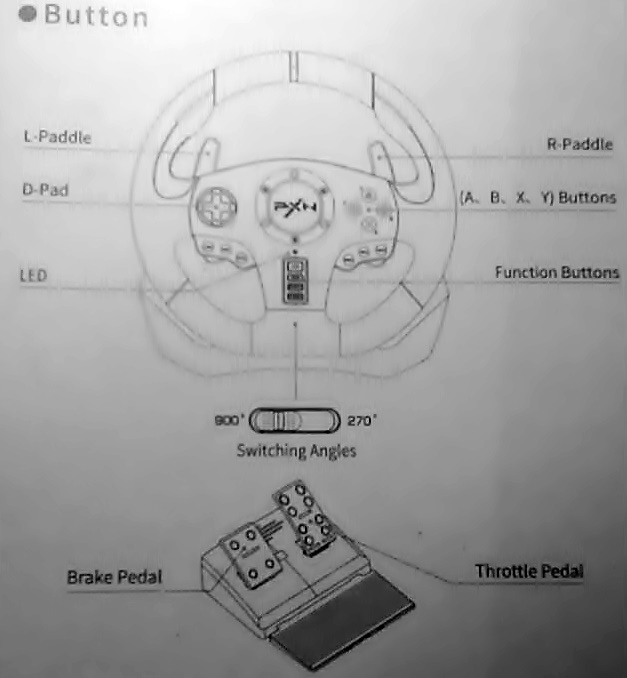
\includegraphics[scale=0.51]{img/steeringwheel.jpg}
	    %\caption{Diagram alur kerja}
	    \caption{Diagram Steering Wheel yang digunakan, \textit{Sumber : Buku Manual PXN Steering Wheel}}
	    \label{fig: 3_28}
    \end{figure}

	Konfigurasi kontroller yang perlu dilakukan adalah salah satunya melakukkan \textit{mapping} tombol - tombol dari keyboard ke tombol - tombol serta perangkat analog dari \textit{steering wheel controller} yang digunakan, seperti contohnya perangkat analog yang perlu dilakukan \textit{sampling} adalah pedal, \textit{sampling} yang dimaksud adalah melakukan pembagian data voltase analog yang ada di pedal menjadi nilai - nilai diskrit yang kemudian dapat dikonversikan ke kecepatan mobil, sesuai nilai - nilai diskrit yang didapatkan. Selain itu juga perlu dilakukan kalibrasi mode sudut dari steering wheel yang memiliki 2 macam mode, yaitu mode 270 derajat putaran, serta 900 derajat putaran. 
	Pada Tugas akhir ini, \textit{steering wheel} akan menggunakan mode 270 derajat, serta proses pergantian gigi \textit{(gear shift)} menggunakan proses manual tanpa kopling. Hal ini dikarenakan keterbatasan perangkat keras yang digunakan.
	
	\begin{figure}  [!htb]
	    \captionsetup{justification=centering}
	    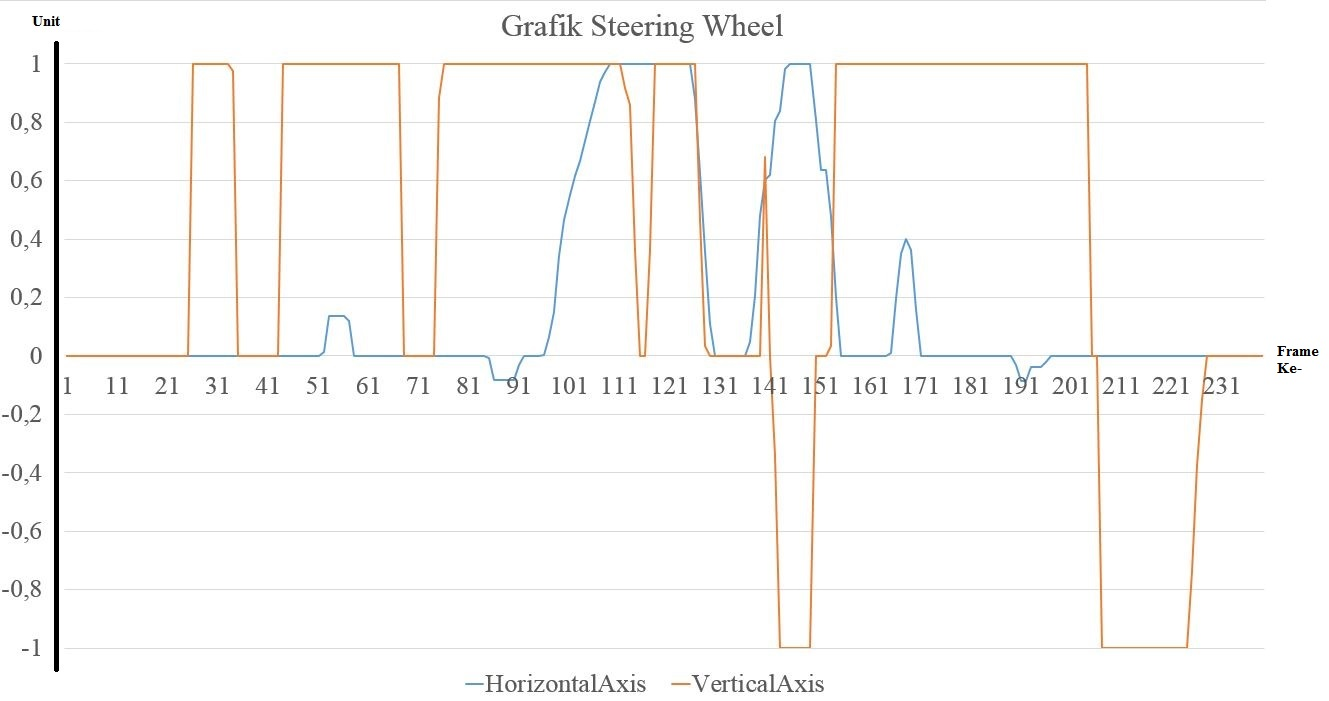
\includegraphics[scale=0.3]{img/driverinput.JPG}
	    %\caption{Diagram alur kerja}
	    \caption{Grafik hasil \textit{plotting} data \textit{input} pengemudi}
	    \label{fig: 3_29}
    \end{figure}
    
    Berikut pada gambar \ref{fig: 3_28} adalah \textit{key map} dari sistem simulator tugas akhir ini. proses kalibrasi pedal gas dan rem disambungkan ke \textit{vertical axis / axis y} dari \textit{unity controller}, maka bisa didapatkan nilai dari pedal atau rem tersebut, berupa data \textit{float} yang memiliki rentang 0 hingga 1. Sedangkan kalibrasi \textit{steering wheel} disambungkan dengan \textit{horizontal axis / axis x} dari \textit{unity controller}, yang memiliki data berupa \textit{float} dengan rentang -1 hingga 1.
    \par Kemudian, data \textit{float} tersebut, dapat dilakukan proses kalkulasi untuk mendapatkan sudut dari pedal gas dan rem, serta sudut dari \textit{steering wheel}, sehingga dapat dilakukan proses \textit{plotting} seperti berikut pada gambar \ref{fig: 3_29}
    
    Selain \textit{vertical axis} dan \textit{horizontal axis}, terdapat pula tombol - tombol lain dari \textit{steering wheel controller} yang digunakan. Yaitu tombol \textbf{X} untuk menyalakan mesin dari mobil \textit{(starter)}, selain itu ada tombol \textit{R-Paddle} dan \textit{L-Paddle} untuk menaikkan dan menurunkan gigi mesin secara berurutan. Proses ini, tidak memerlukan kopling, cukup menekan tombol \textit{L-R-Paddle} untuk menaikkan atau menurunkan gigi mobil.
    
    \par Di tengah \textit{steering wheel} juga terdapat \textit{switch} untuk mengganti mode \textit{steering} yaitu mode 270 derajat atau 900 derajat.
\section{Pembuatan Modul Pengambilan Data dengan \textit{Microcontroller}}
\label{microcontroller}
\vspace{1ex}

    \begin{figure}  [!htb]
	    \captionsetup{justification=centering}
	    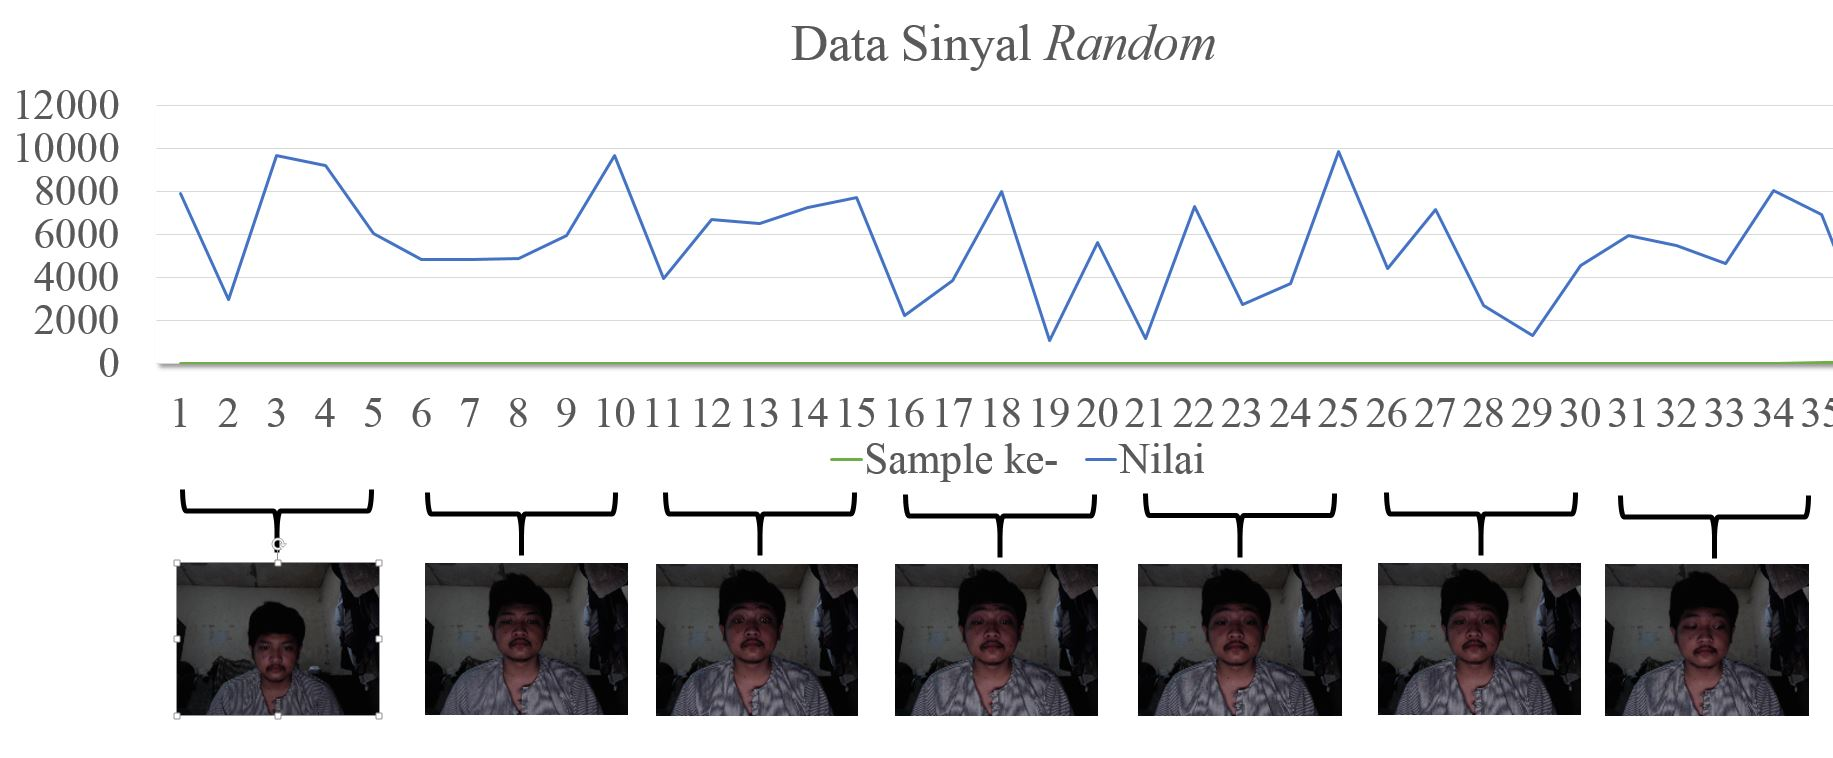
\includegraphics[scale=0.2]{img/sinyaldangambar.JPG}
	    %\caption{Diagram alur kerja}
	    \caption{Diagram Sinkronisasi \textit{capture rate} kamera dengan \textit{sampling rate} dari sensor arduino}
	    \label{fig: 3_30}
    \end{figure}
    
    Pembuatan modul pengambilan data serial seperti EEG dan ECG, dapat dilakukan menggunakan Arduino, sehingga perlu disiapkan port USB. Sedangkan pengambilan data berupa gambar wajah pengemudi menggunakan kamera, dapat disambungkan langsung ke \textit{Unity Game Engine} dan dapat langsung disimpan ke \textit{harddrive} komputer simulator. Hal ini dilakukan agar data yang masuk berupa gambar wajah pengemudi serta sinyal - sinyal yang di peroleh oleh \textit{microcontroller} dapat di lakukan pengolahan dan proses analisa.
    Perlu di perhatikan juga \textit{sampling rate} dari sistem pengambilan sinyal arduino, dengan \textit{capture rate} dari \textit{webcam}, kedua data tersebut perlu di sinkronkan dengan memperhatikan kedua nilai tersebut. \textit{Sampling rate} dari arduino disini bisa didapatkan dari \textit{datasheet} sensor yang digunakan, kemudian dilakukan kalkulasi dengan \textit{margin of error} yang disebabkan oleh kegagalan transmisi data dari arduino ke komputer simulator melalui kabel USB, agar didapatkan hasil yang dapat diterima. Sedangkan \textit{capture rate} dari kamera merupakan seberapa banyak gambar atau \textit{frame} yang diambil oleh kamera tiap \textit{frame} yang di proses oleh simulator. Pada Tugas Akhir ini, target capture rate adalah 1:1. Yang artinya, kamera akan mengambil gambar wajah pengemudi tiap frame game tersebut dijalankan. Berikut pada gambar \ref{fig: 3_30} adalah diagram dari penjelasan sinkronisasi kedua data tersebut, menjadi suatu modul analisis sinyal dengan gambar wajah.
    
\section{Penggabungan Seluruh Sistem Menjadi Satu Modul}
\vspace{1ex}
    Langkah terakhir adalah mengintegrasikan seluruh sistem menjadi satu modul yang utuh, supaya dapat melakukan pengolahan data dengan irisan waktu \textit{(t)} yang bersamaan. Keluaran yang diharapkan adalah, simulator dapat melakukan pengambilan data analog, data citra gambar, serta data - data internal simulasi secara bersamaan dan integrasi. Seperti yang dijelaskan pada bab \ref{logfilesystem} hingga bab \ref{steeringwheelconf}, Penggabungan Sub - sub modul, menjadi satu modul utuh adalah seperti berikut
    
    \begin{enumerate}[nolistsep]
	
	\item Sub-modul pengambilan data internal, mencakup :
	    \begin{enumerate}[nolistsep]
	        \item Sub-Modul Kecepatan Mobil
	            \begin{enumerate}
	                \item Kecepatan Vektor Sumbu \textit{x,y,z}
	                \item \textit{Magnitude} Kecepatan Vektor
	            \end{enumerate}
	        \item Sub-Modul Informasi Spasial
	            \begin{enumerate}
	                \item Posisi Relatif Mobil terhadap jalan
	                \item Sudut Euler dan \textit{6 Degree of Freedom} - Pitch, Yaw, Roll
	            \end{enumerate}
	        \item Sub-Modul Respon Pengemudi
	            \begin{enumerate}
	                \item Informasi Respon Pengemudi Ketika kendaraan keluar jalur
	                \item Informasi \textit{Input} dari Steering Wheel Controller (Sudut \textit{Steering Wheel} dan Nilai Tekanan Pedal Gas dan Rem)
	            \end{enumerate}
	    \end{enumerate}
	\item Sub-modul pengambilan data eksternal, mencakup :
	    \begin{enumerate}[nolistsep]
	        \item Sub-Modul Sinyal dan Citra Wajah
	            \begin{enumerate}
	                \item Sinyal dari sensor, bisa berupa ECG, EEG, atau EOG
	                \item Citra Wajah tiap frame dari kamera
	            \end{enumerate}
	    \end{enumerate}
	
	\end{enumerate}
    
Pada tugas akhir ini, sub - sub modul dibentuk berdasarkan kebutuhan proses pengujian, namun untuk riset kedepannya, proses pembuatan serta sinkronisasi data - data sub-modul bisa dapat dilakukan penyesuaian sesuai dengan kebutuhan riset tersebut yang menggunakan data dari simulator ini.
    
    
    
% GAMBAR KALIBRASI STEERING WHEEL
%\begin{figure} [!htb]
%	\captionsetup{justification=centering}
%	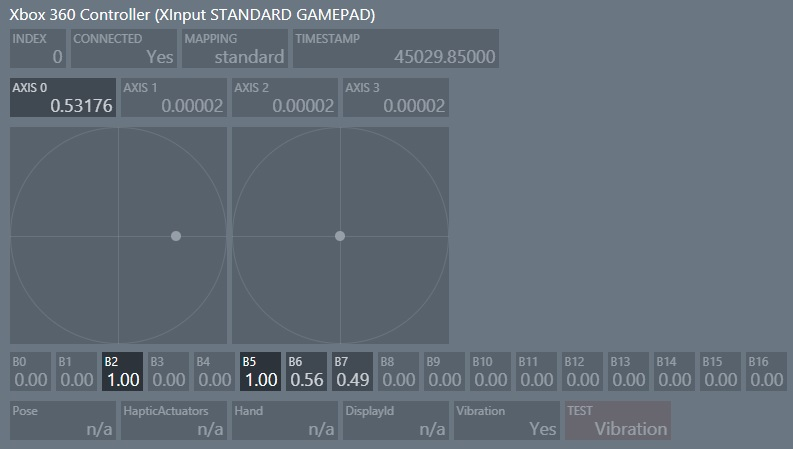
\includegraphics[scale=0.5]{img/steering-wheel-calibration.jpg}
%	\caption{Informasi Steering Wheel }
%	\label{fig: 3_7}
%\end{figure}

%GAMBAR FLOW CHART KOMUNIKASI PYTHON
\begin{figure}  [!htb]
	        \captionsetup{justification=centering}
	        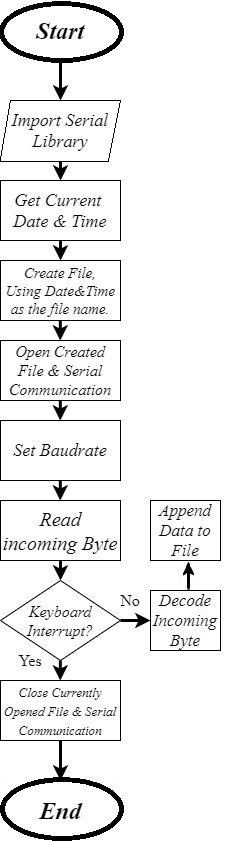
\includegraphics[scale=0.7]{img/serial-comm.jpg}
	        \caption{Diagram \textit{Flow Chart} Komunikasi Serial Melalui \textit{port} COM}
	        \label{fig: 3_25}
\end{figure}